\documentclass[12pt]{article}

\usepackage{a4}
\usepackage{fullpage}
\usepackage{graphicx}
\usepackage{float}
\usepackage[bahasa]{babel}
\usepackage[font=small,labelfont=bf]{caption}

\setlength{\parskip}{1em}
\setlength{\parindent}{4em}
\tolerance 9999 \emergencystretch 3em\relax

\makeatletter
\newcommand{\chapterauthor}[1]{%
  {\parindent0pt\vspace*{-10pt}%
  \linespread{1.1}\small\scshape#1%
  \par\nobreak\vspace*{10pt}}
  \@afterheading%
}
\makeatother

\begin{document}
    \section*{Sejarah dibalik Era Kompetitif \emph{Counter-Strike: Global Offensive}}
    \chapterauthor{ditulis oleh Rivo Juicer Wowor}
    
    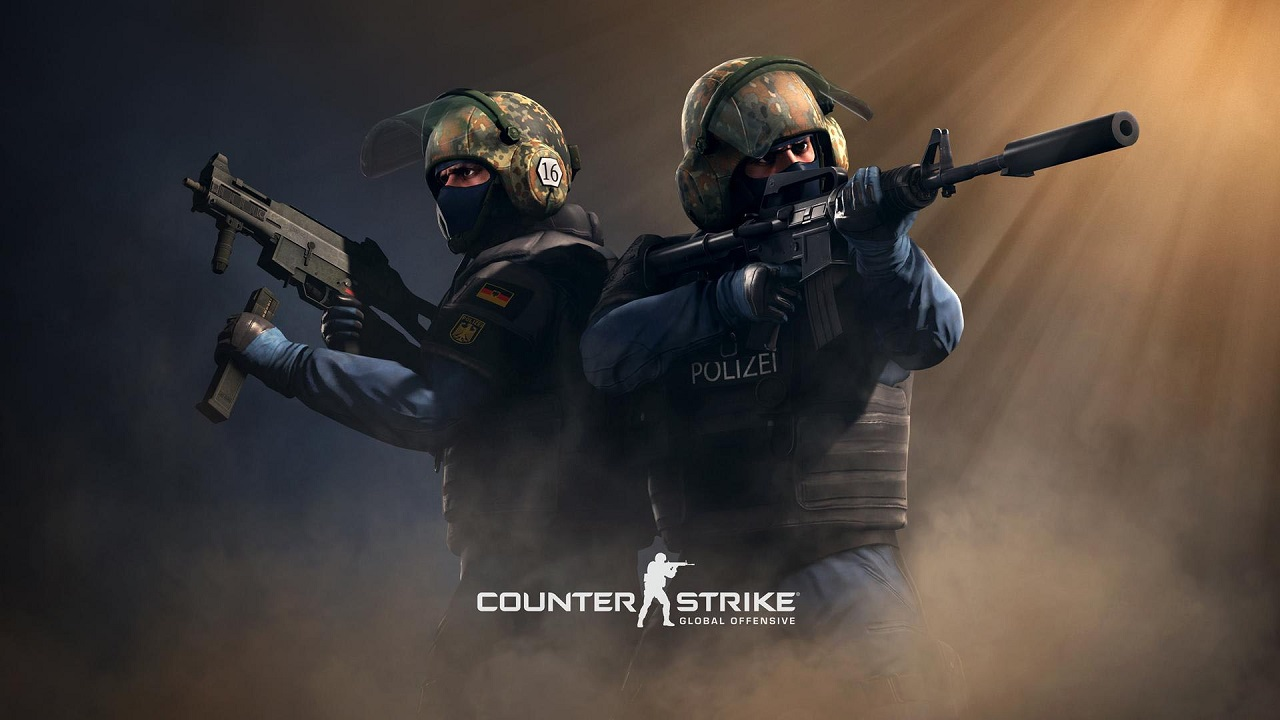
\includegraphics[width=1.0\textwidth]{images/csgo-1.jpg}
    \vspace{1pt}

    \emph{Counter-Strike: Global Offensive} adalah sebuah permainan video
    untuk Windows, Mac, dan Linux yang dirilis pada tahun 2012. Permainan
    ini merupakan salah satu dari seri \emph{Counter-Strike} yang telah ada
    sejak tahun 1999. \emph{Counter-Strike} juga merupakan salah satu cabang
    olahraga \emph{eSports} atau olahraga elektronik. Banyak turnamen yang
    diselenggarakan untuk cabang olahraga ini. Contohnya seperti \emph{ESL
    One Cologne, ESL Pro League, BLAST Premier, Dreamhacks Open,} dan juga
    \emph{FACEIT Pro League}.

    \emph{Counter-Strike} memiliki sejarah kompetitif selama 20 tahun yang
    dimulai pada versi awal \emph{Counter-Strike}. Salah satu turnamen
    \emph{Major} (seperti Piala Presiden dalam sepak bola) pertama yang
    diselenggarakan yaitu \emph{Cyberathlete Professional League Winter
    Championship} pada tahun 2001 dan dimenangkan oleh tim \emph{Ninjas in
    Pyjamas} dari Swedia. Dari saat itu, perkembangan olahraga elektronik
    \emph{Counter-Strike} mulai berkembang pesat. Seperti munculnya Liga
    \emph{World Cyber Games} dari Korea, liga \emph{Cyberathlete
    Professional League} dari tahun 2001 hingga 2006, hingga \emph{ESL Pro
    League} dari tahun 2015 hingga Sekarang

    \begin{figure}[H]
    \centering
    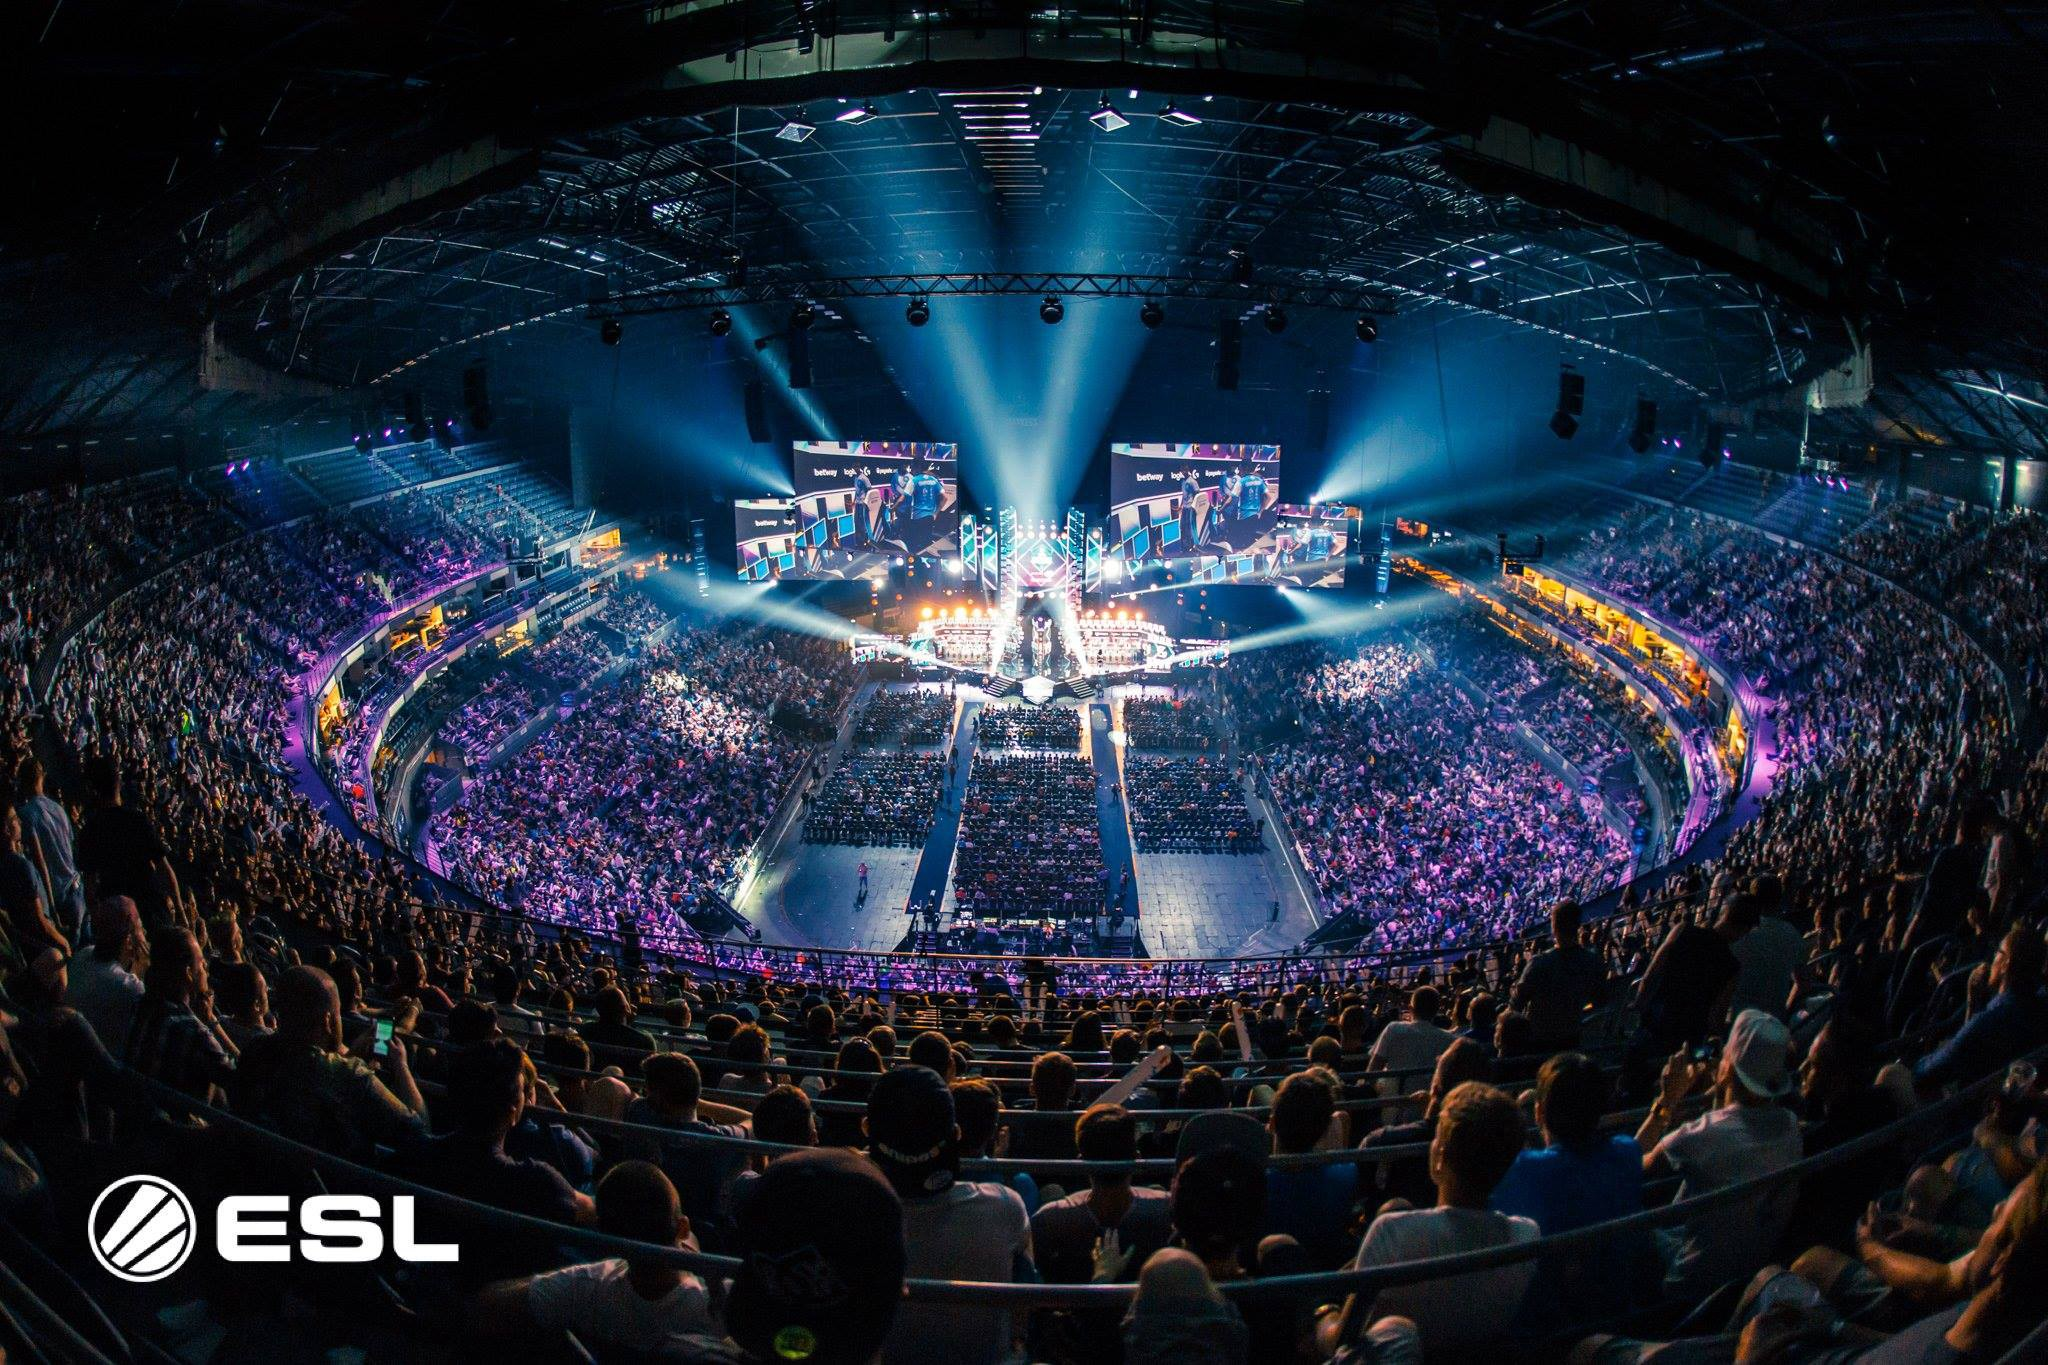
\includegraphics[width=1.0\textwidth]{images/1_qkFJj0JlKig9wgiNKYMJCg.jpeg}
    \caption{Salah satu turnamen terbesar di sejarah Counter-Strike, ESL One
    Cologne}
    \end{figure}

    Valve, perusahaan yang membuat permainan \emph{Counter-Strike} kesulitan
    dalam mengembangkan versi pertama \emph{Counter-Strike} dikarenakan
    tingkat \emph{skill} yang cukup tinggi untuk pemain-pemain baru. Oleh
    karena itu pada tahun 2004, Valve merilis \emph{Counter-Strike: Source}.
    Tapi hal ini justru membuat komunitas dari \emph{Counter-Strike}
    mengkritik perbuatan Valve tersebut, dikarenakan Valve terlalu
    memudahkan game tersebut sehingga rasa kompetitifnya telah hilang
    dibandingkan versi pertama \emph{Counter-Strike}. Dan dari hal tersebut,
    komunitas \emph{Counter-Strike} terpecah menjadi dua.

    Setelah beberapa tahun, akhirnya pada tahun 2012 Valve merilis
    \emph{Counter-Strike: Global Offensive}. Awalnya perilisan permainan ini
    justru mendapat banyak kritikan dari komunitas \emph{Counter-Strike}.
    Tapi setelah beberapa lama dan juga dedikasi dari Valve dalam
    mengembangkan permainan ini, komunitas yang awalnya terpecah menjadi
    dua, kembali bersatu karena game ini. Rilisnya game ini juga bertepatan
    dengan naiknya popularitas website \emph{game streaming} seperti
    \emph{UStream, Justin.tv} dan \emph{Twitch} yang membuat sisi olahraga
    dari Counter-Strike ini naik daun.

    \begin{figure}[H]
    \centering
    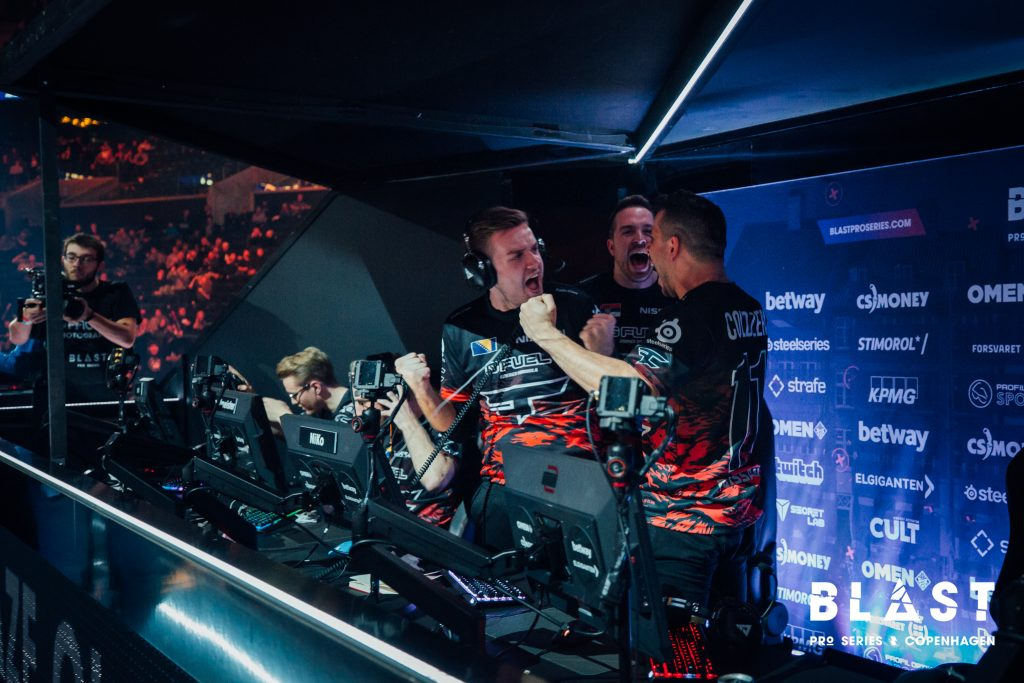
\includegraphics[width=1.0\textwidth]{images/20191102_Adela-Sznajder_BLASTProSeriesCPH_04183-1024x683.jpg}
    \caption{FaZe Clan ketika memenangkan liga BLAST Pro Series 2020 pada
    Januari lalu}
    \end{figure}

    Hingga saat ini, \emph{competitive scene} dari \emph{Counter-Strike:
    Global Offensive} masih sangat populer dikalangan olahraga eSports.
    Meskipun dengan banyaknya kontroversi dan juga masalah yang terjadi
    belakangan ini, komunitas dari \emph{Counter-Strike} tetap setia dalam
    mengikuti olahraga ini. Dan dengan jumlah pemain yang bertanding
    mencapai satu juta per harinya, Saya rasa \emph{Counter-Strike} akan
    terus berkembang menjadi salah satu game terbesar dan tertua dalam
    sejarah \emph{eSports}.
\end{document}